\documentclass[oneside]{tum-book}

\usepackage{subcaption}

\title{Cotton Candy Digital Twin: Prescriptive Creation of Digital Twins}
\germantitle{Titel der Abschlussarbeit}
\author{Nicolás Mario Arteaga García}

\chair{Chair of Information Systems and Business Process Management (i17)}
\school{TUM School of Computation, Information and Technology}
\department{Department of Computer Science}
\thesistype{Master's Thesis in Informatics}
\degree{Master of Science}

\examiner{Prof. Dr. Stefanie Rinderle-Ma}
\supervisor{Dr. rer. soc. oec. Juergen Mangler}

\hood{Garching}
\submissiondate{31.07.2025}

\begin{document}
  \chapter*{Abstract}
\noindent
150 - 180 words 


\textit{\textbf{Keywords: Digital Twin, Cotton Candy, BPTM, Data Collection, Data Science} \\Include three to five words, phrases, or acronyms as keywords.}

  
  \newpage

  \tableofcontents
  \listoftables
  \listoffigures
  \newpage

  \chapter{Introduction}
\label{sec:intro}

For exposes, create this chapter, plus start with chapter 2 (Related Work).

\section{Motivation}
\label{sec:intro:mo}

Why are we doing it? About 1 page.

As industries evolve, the ability to optimize processes while minimizing waste has become increasingly important. Digital twins (virtual models of physical systems) are transforming how we monitor, analyze, and improve these processes. While reactive digital twins respond to events as they occur, providing immediate but limited feedback, predictive digital twins forecast potential outcomes based on historical and real-time data, allowing proactive adjustments. However, the growing focus on prescriptive digital twins introduces a new frontier: systems that not only predict outcomes but also recommend specific actions to achieve goals such as improving efficiency, reducing energy consumption, or enhancing product quality.

This thesis explores the development of prescriptive digital twins using the Cotton Candy Automata, a robotic system developed in the chair to automate cotton candy production, as a practical and measurable test case. This scenario provides an ideal environment for evaluating two distinct approaches to digital twin design—bottom-up and top-down—by analyzing key variables such as heating time, spinning duration, sugar amount, and energy usage. Each approach takes a unique perspective:

Bottom-Up Approach: Focuses on physical measurements and process models, leveraging real-time sensor data to guide system optimization.

Top-Down Approach: Relies on historical data and advanced computational methods, including interpolation, selection of closest historical values, and machine learning models like Recurrent Neural Networks (RNNs), to model and optimize the system.

The goal of this thesis is to provide a comprehensive evaluation of these two approaches, comparing their strengths, limitations, and suitability for different scenarios. By analyzing metrics such as energy savings, time efficiency, and production quality, the research aims to determine which method offers the greatest value (for this process/for specific process types?). Applying both methodologies to the same scenario enables a deeper understanding of their trade-offs and practical implications, offering insights that can guide future efforts in digital twin development.

Ultimately, this work contributes to the broader understanding of how to design and implement prescriptive digital twins, providing actionable recommendations for selecting the best approach based on system goals, constraints, and operational contexts.

\section{Research Questions}
\label{sec:intro:rq}

At least 3 questions. They should not be answerable yes/no. Questions should be
questions (1 sentence). But you are allowed to explain them in more detail. In
the explanation also tell how you plan to prove that your potential future
solution is good.

About 1 page.

Fexamples: 
(1) How can we design and implement prescriptive digital twins for the Cotton Candy Automata?
(2) MMM What are the strengths and limitations of each approach, and how do they impact key metrics such as energy savings, time efficiency, and production quality?

\section{Contribution}
\label{sec:intro:con}

What will/have I do/done that nobody else has done before. About 1/2 page.

\section{Methodology}
\label{sec:intro:meth}



Design Science in Information System (Hevner). How are we doing research?

(1) Summary what design science is (it uses stakeholders, artefacts, steps,
...). 

(2) What are the stakeholders, artefacts, steps for MY case.
What does it mean for my thesis?

About 1.5 pages.

% Stichpunkte:
% - Use Hevner's framework to justify Design Science as methodology
% - You're building and evaluating a technical artefact (digital twin + quality assessment)
% - Real-world relevance: improving cotton candy production
% - Scientific rigor: structured measurement and evaluation
% - Matches Hevner's cycle: build → evaluate → improve

This work follows the Design Science Research (DSR) paradigm as defined by Hevner et al.~\cite{Hevner2004}. The DSR approach provides a structured framework for the development and evaluation of innovative artefacts that solve real-world problems in a rigorous and methodologically grounded manner.

In the context of this thesis, the central artefact is a digital twin system for a cotton candy production robot. This artefact comprises both the virtual representation of the physical process and the accompanying infrastructure for capturing environmental and process-related parameters (e.g., humidity, input sugar, and runtime), as well as metrics of product quality (e.g., volume, weight, and fluffiness).

The digital twin is iteratively refined through cycles of design and evaluation, in accordance with the DSR methodology. The system is deployed in a real-world production context and evaluated based on its ability to improve product quality and production efficiency under varying conditions. This dual focus on practical applicability and measurable improvement ensures that the artefact addresses both relevance and rigour — the core criteria of Hevner’s framework.

\section{Evaluation}
\label{sec:intro:ev}

How will I evaluate that my proposal is good. This ties into the research questions.

About 1 page.

\section{Structure}
\label{sec:intro:struct}

Which chapters will my thesis have, and what are they all about.
About 1/4 page.

  \chapter{Related Work}
\label{sec:rel}

Related Work - There is a girl with long dark hair doing a thesis on digital twin as a research analysis. ask her per discord

google scholar in-title digital twin / business processes, search queries that give you less than 20 papers and decide 1 or 2 papers in the end. How many papers did we eliminate? why? bc too

backgorund 1-2 sentences
-> Why am I doing something different to this related work

Final max 4-5 papers that really relate to what Im doing


THis one doesnt work bc, its for bridges and civil engineering
https://www.sciencedirect.com/science/article/pii/S0141029623017984

this one looks good :
https://www.sciencedirect.com/science/article/pii/S0360835224003620

\section{Thermal Study on Cotton Candy}
Cotton candy consists of spun sucrose that cools rapidly, forming a mostly amorphous structure — but:
	•	Over time, this amorphous state can convert into crystalline form.
	•	The ratio between crystalline and amorphous sucrose affects:
	•	Texture
	•	Stability
	•	Taste
	•	Shelf-life

% The paper investigates how the physical structure of cotton candy changes depending on how it is produced and stored, focusing especially on how much is amorphous vs crystalline sucrose.
% 	•	The author studies this using Differential Scanning Calorimetry (DSC), a thermal analysis technique to measure transitions like glass transitions, crystallization, and melting.
% 	•	The novelty: the study compares cotton candy spun in air vs in nitrogen atmosphere to see how different gas environments affect its physical and thermal properties.

% In essence, it’s a study of the physics of sugar in cotton candy — very relevant to your Cotton Candy Automata project, as this kind of data gives insight into the material side of your digital twin.

This paper provides very solid experimental data on how production parameters influence the physical structure (crystalline vs amorphous) of cotton candy.

Crystalline is \dots
Amorphous is \dots

% Because the amorphous vs crystalline ratio affects:
% 	•	Shelf life (amorphous recrystallizes over time)
% 	•	Stability (stickiness, collapse, hardening)
% 	•	Thermal behavior (different melting/glass transition points)
% 	•	Quality (texture, mouthfeel)

Knowing how production parameters (like gas environment) affect structure can inform optimal production recipes. We are not gonna compare CCA vs CCN, since we are always using Normal Air but
We learn about the importance of humidity, and want to use it for our Data Recollection since this is important For the Prescriptive twin design.

This helps with us taking the decision how to measure the quality of CC when doing data recollection and giving a note to the process.

What makes it difficult is that the changes are fine and little, and we dont really know if we are gonna be able to distinguish them, but we did research and will introducte this in the Solution Design.

% Smooth operatoooor



  \chapter{Solution Design}
\label{sec:solution}

    •	What is the physical structure of cotton candy?
    What aspects define “quality” of cotton candy?     •	What are the key factors that affect quality?
    •	How does it change with production parameters?
    What we already learned doing cc is -> The notes from the notion

\section{    •	What is the physical structure of cotton candy?}
Cotton candy is primarily composed of spun sucrose, which can exist in two main forms:WHat we saw in the paper\dots

\section{What aspects?}

YES: Volume density -> How much sugar is in a given volume -> Weighing sample and measuring volume (water displacement) => Doing this wiht a trichter that has the exact volume written. How does it change wiht more or less humidity?

NO: Visual appearance -> Fiber structure, color, consistency -> Visual inspection, photography + image analysis (even with your phone and Python/OpenCV) => we are not gonna do this because we learned that it is not really possible to distinguish the fibers with the naked eye. Its a full master thesis on its own

NO: Texture \& mouthfeel -> Stickiness, softness, “melt-in-mouth” -> Manual touch test, break force => Stickiness is interesting to measure but probably difficult more on it later 
NO: Hygroscopic behavior -> Stickiness as it absorbs moisture -> Weighing sample over time at room humidity => This is very interesting, takes time to measure but hey -> NO BC WE WILL CREATE THEM IN DIFF ENVIRONMENTS AND CANNOT CREATE A CONTROL CAPSULE

YES: Crispness vs softness -> Related to crystallinity -> Compression test (kitchen scale or small force sensor) => It would mean measureing how much compression force is needed to break the fibers, very difficult, we build a model that we could test between CC and after measuring volume we weighted it, we tested this and that and concluded\dots

 B. Compression Test
	•	Use a small kitchen scale or force sensor.
	•	Press gently until collapse starts.
	•	Record maximum weight/force applied.
	•	Amorphous cotton candy tends to be softer; more crystalline samples resist compression.
% ➡ Proxy for structure & texture.

NO: Structural stability -> How long it holds shape over time -> Timed visual check at room conditions => Takes long to test, 

NO: Taste (subjective) -> Flavor preception is too subjective so we will not do this, but it is important to note that it is a factor in quality perception.

\section{    •	How does it change with production parameters?}
How can we change the environment and control so that production parameters are changed 
    •	Humidity: Higher humidity leads to more stickiness and faster recrystallization. -> How to simulate Humidity?
    The gas environment during spinning directly changes how much of the sucrose becomes crystalline vs amorphous.
	•	More oxygen \& moisture → more crystallization.
	•	Less oxygen \& low moisture (like nitrogen or dry air) → more amorphous content.
    -> We cannot change the environment, but we can change the humidity of the process with:
        - Airflow / fans -> Stronger air movement near spinner -> Helps dry fibers during flight/creation, reduces moisture pickup.
    -> YESSSS LETS DO THIS

    % IMPORTANt
    Affect on more humidity durign spinning -> Fibers may break sooner, become shorter, thicker. fibers stick together more.
    and after spinning -> Fibers collapse and shrink, Loss of volume (shrinkage), stickiness increases. what about compression?
    Immediately after spinning (fresh)
- Fibers in humid air are thicker, stickier → denser structure → higher compression resistance initially (less fluffy, more “compact”). - Less air trapped between fibers → more force needed to compress.
Shortly after spinning (as moisture is absorbed)
- As fibers absorb moisture, they soften → compression force quickly drops. - Structure collapses under small loads.
% IMPORTANt

Compression is kind of complicated to test since: 
Actually, at high humidity:
	•	At first → more compact = higher compression resistance.
	•	But as time passes → absorbs moisture → weaker structure = lower compression resistance.

In contrast, at low humidity:
	•	The fibers stay dry, fluffy, and light.
	•	Lower compression resistance but much better structural stability over time.

    Humidity Level
        Result that we think we could achieve:
        Low RH \(<30\%\)
        Light, fluffy, large volume, fine fibers.
        High RH \(>60\%\)
        Denser, smaller volume, coarser fibers, faster shrinkage.


    •	Temperature: Higher temperatures can lead to more amorphous structure, but too high can cause burning. We have no control over this, as we are gonna see in the Solution Design, we are using a machine that always stays at the same ratio of temperature when at work. 
    -> What we can control and change is the Cooking time, so the temperature that the head had when inserting the suagr and the time that we let the cotton candy get created, and let the arm roll. -> What this hopefully gives us is the change in structure that we can test with the compression test and a bigger volume.

    •	Spinning speed: Faster spinning may lead to finer fibers, affecting texture. Spinning speed (Higher RPM) Creates finer fibers, helps counteract thickening effect of humidity. -> We cannot control this. The given machine always spins in the same speed.

    -  One big variable that I had at the start was the Sugar amount. Thinking naively, I thought that more sugar would lead to more volume, but this is not the case. The amount of sugar in the process is always the same, and we are not changing it. We are always using the same amount of sugar for each production, which is 10 grams. -> Adding more won’t help volume, might increase stickiness. And we are not measuring this change in stickiness as we saw before.

    - Sugar formulation -> Use anti-hygroscopic additives (e.g., small \% of maltodextrin or stabilizers) -> Slows moisture absorption. Often used in industrial production. We are not chanign the sugar formulation. We are always using the same sugar from the supermarket for making it easier to reproduce the results.

\section{What we learned empirically doing CC}
    - write times, forms, radius why that radius etc etc etc

    => We can create a formula of how we think it behaves, that we can compare afterwards in the Data Recollection Evaluation.

\section{Prescriptive Digital Twin Flow}

- We have an Environment that we cannot control, but we can measure it.
- We have a process that we can control, but what exactly? THe time of cook? (Yes) The amunt of sugar? (Yes, but doesnt impact), The heating up before spinning? (Yes, but only energy savings impact) The \dots
- We have a product that we can measure and evaluate the quality, but how? (First measure the Volume and then the compression stress, etc) 

With 200 points of this data we can create a Model that can forecast the quality mark of the product looking at the ENV and the Process Rules. With Desicion Trees since this and that\dots

With the Forecasting we can change the Process rules to imporve the quality of the product. How? With Decision Trees? Trasvering back? How should it be done? I dont know yet.




\begin{figure}[h]
    \centering
    \caption{My Figure Caption}
    
\includegraphics[width=0.7\textwidth]{tum-resources/images/Universitaet_Flaggen.jpg}
    \floatfoot{A note describing the figure}
    \label{fig:firstFigure}
\end{figure}

  \chapter{Implementation}
\label{sec:implementation}

\section{Automata}
TODO What we learned when we created the automata and the simple function that we are gonna use for data collection.

\subsection{Sugar Amount}\label{subsec:sugar-amount}
To calibrate the sugar dispensing system, we measured ten times the amount of sugar released over durations of 0.5s, 1s, 1.5s and 2s (2s slightly overflowed the spoon)with each setting tested in multiple trials. The resulting median values were 8.50g, 12.63g, and 16.64g, 20.58g respectively. These findings confirmed a roughly linear relationship between dispensing duration and sugar quantity. For all subsequent trials and modeling efforts, we standardized the input to 1s of sugar dispensing so 12.63g.

\subsection{Waiting Time}
The time the robot arm waits until sugar starts flowing out of the spinner. The cold start time was a variable used for the first time (102s) with an environment of ~25C, our digital twin will leave this variable unneeded. Since it will already know how to act with the actual temperature of the spinner.
At the end of the thesis we will see the variance of this time, based mostly on how warm the spinner will be before.

\subsection{Cooking Time}
The default cooking time is 105s. This starts once the sugar starts flowing out of the spinner. probably becauase the spinner has reached the desired temperature for more than (10-20 seconds). (TODO: Be sure about this)
The spinning time is always 3.75s.
105/3.75 = 28 spins per run.

\subsection{Cooldown Time}
The cooldown time is the time that the spinner runs without the heat, to cool down after the production run. This is needed to avoid burning the sugar in the next run. The default cooldown time is 60s, but we are gonna research how good the quality is gonna be if we increase or decrease this value. 
The Machine manual empfehlen to wait 120s, but we started with 60s bc we noticed a lot room for improvement while using the automata and sometimes it takes a long time to start the next process again to put the sugar and turnon the machien again makes it roughly 120s anyway.

\subsection{Cotton Candy iteration}
We are gonna store which cotton candy iteration we are on, since the last time the machine has been cleaned. We already noticed what a big difference it can make on the quality when the machine has run for a long time without cleaning. 
We want to find the optimal value of iterations we want to run before cleaning the machine. We will start with max 20 iterations.
We will clean the machine and declog the sugar of the spinner with water.


\section{Energy Consumption Measurement}
\label{sec:energy-measurement}

Energy consumption is measured and stored for each production cycle to enable optimization of process parameters for energy efficiency. This measurement, combined with quality metrics, allows the digital twin system to find optimal parameter settings that minimize energy consumption while maintaining product quality.

\subsection{Data Acquisition and Calculation}

Power consumption is measured using a smart plug at 2-second intervals throughout the production process. Total energy consumption is calculated using trapezoidal integration of discrete power measurements:

\[
E = \sum_{i=1}^{n} \frac{P_{i-1} + P_i}{2} \cdot \Delta t_i
\]

where $P_i$ is the power measurement at time $t_i$ and $\Delta t_i$ is the time interval between measurements. The result is converted from Watt-seconds to Watt-hours for practical interpretation of the 5-minute production cycles.

This methodology captures energy consumption across all production phases (startup, heating, spinning, cooldown) and provides the optimization target for energy-efficient cotton candy production.

% \subsection{Power Data Acquisition}
% 
% Power consumption data is collected using a smart plug (Tasmota-compatible device) that measures electrical parameters at 2-second intervals throughout the production process. The plug captures instantaneous power values in Watts, which are logged with precise timestamps in the process execution system (XES) format. Given the short duration of cotton candy production (maximum 5 minutes), this sampling frequency provides sufficient temporal resolution for accurate energy integration.
% 
% \subsection{Energy Calculation Methodology}
% 
% Total energy consumption for each production cycle is calculated using trapezoidal numerical integration of the discrete power measurements over time. This approach accounts for the varying power draw during different phases of the cotton candy making process (heating, spinning, cooling).
% 
% The energy calculation follows the fundamental relationship:
% \[
% E = \int_{t_0}^{t_f} P(t) \, dt
% \]
% 
% where $E$ is the total energy consumed, $P(t)$ is the instantaneous power at time $t$, $t_0$ is the process start time, and $t_f$ is the process end time.
% 
% For discrete measurements taken at intervals $\Delta t = 2$ seconds, the trapezoidal rule approximates this integral as:
% 
% \[
% E \approx \sum_{i=1}^{n} \frac{P_{i-1} + P_i}{2} \cdot \Delta t_i
% \]
% 
% where:
% \begin{itemize}
%     \item $P_i$ is the power measurement at time $t_i$
%     \item $\Delta t_i = t_i - t_{i-1}$ is the time interval between consecutive measurements
%     \item $n$ is the total number of measurement intervals
% \end{itemize}
% 
% The result is expressed in Watt-seconds (Joules), which is then converted to Watt-hours by dividing by 3600:
% 
% \[
% E_{Wh} = \frac{E_{Ws}}{3600}
% \]
% 
% For the typical 5-minute cotton candy production process, Watt-hours provide a more intuitive unit than kilowatt-hours, which would result in very small decimal values.
% 
% \subsection{Process Phase Integration}
% 
% The energy calculation spans the complete production cycle, from process initiation to final cooldown. Key phases include:
% 
% \begin{enumerate}
%     \item \textbf{Startup phase}: Initial power draw as the spinner begins heating
%     \item \textbf{Heating phase}: High power consumption to reach operating temperature
%     \item \textbf{Production phase}: Active spinning and sugar melting with varying power draw
%     \item \textbf{Cooldown phase}: Reduced power consumption during cooling period
% \end{enumerate}
% 
% By integrating power consumption across all phases, the methodology captures the total energy cost of each cotton candy unit, enabling optimization of process parameters for energy efficiency while maintaining product quality.
% 
% \subsection{Data Quality Considerations}
% 
% The trapezoidal integration method assumes linear interpolation between discrete measurement points. While this introduces some approximation error, the 2-second sampling interval is sufficiently fine-grained relative to the thermal and mechanical time constants of the cotton candy machine to provide accurate energy estimates. Additionally, the method handles variable time intervals between measurements, accommodating any minor variations in data logging frequency.

\subsection{Weight Measurement} 

% Stichpunkte:
% - Manually weigh sugar before each run (input)
% - Weigh finished cotton candy on stick
% - Subtract known stick weight to get net cotton candy weight
% - Use same digital scale throughout
% - Needed for yield and fluffiness index

The input mass of sugar for each production run was manually measured using a precision scale with a readability of 0.01 grams. To determine the output mass of the produced cotton candy, the final product (including the stick) was weighed immediately after production using the same scale. The net weight of the cotton candy was then computed by subtracting the known weight of the stick, which was measured prior to the experiment and kept constant across all runs.

Accurate weight measurement was essential for evaluating the amount of produced cotton candy and for computing derived metrics such as the quality and Fluffiness Index. All weights were recorded in grams with a precision of two decimal places.



% TODO: Change Image to a better and smaller one, this is just a placeholder
% \begin{figure}[H]
%         \caption{Comparison between geometric approximation and real cotton candy morphology}
%     \label{fig:volume-comparison}
%     \centering
%         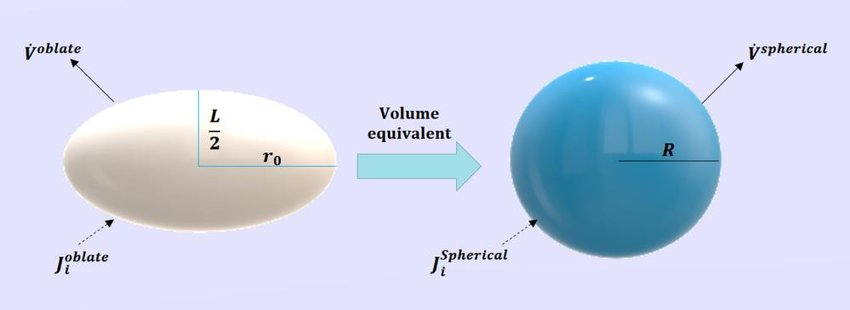
\includegraphics[width=\textwidth]{figures/Schematic-diagram-of-the-oblate-spheroid-and-its-volume-equivalent-sphere.jpg}
%         % \caption{Idealized oblate spheroid}
%         \label{fig:oblate-spheroid}
% \end{figure}
% \begin{figure}[H]
%         \centering
%         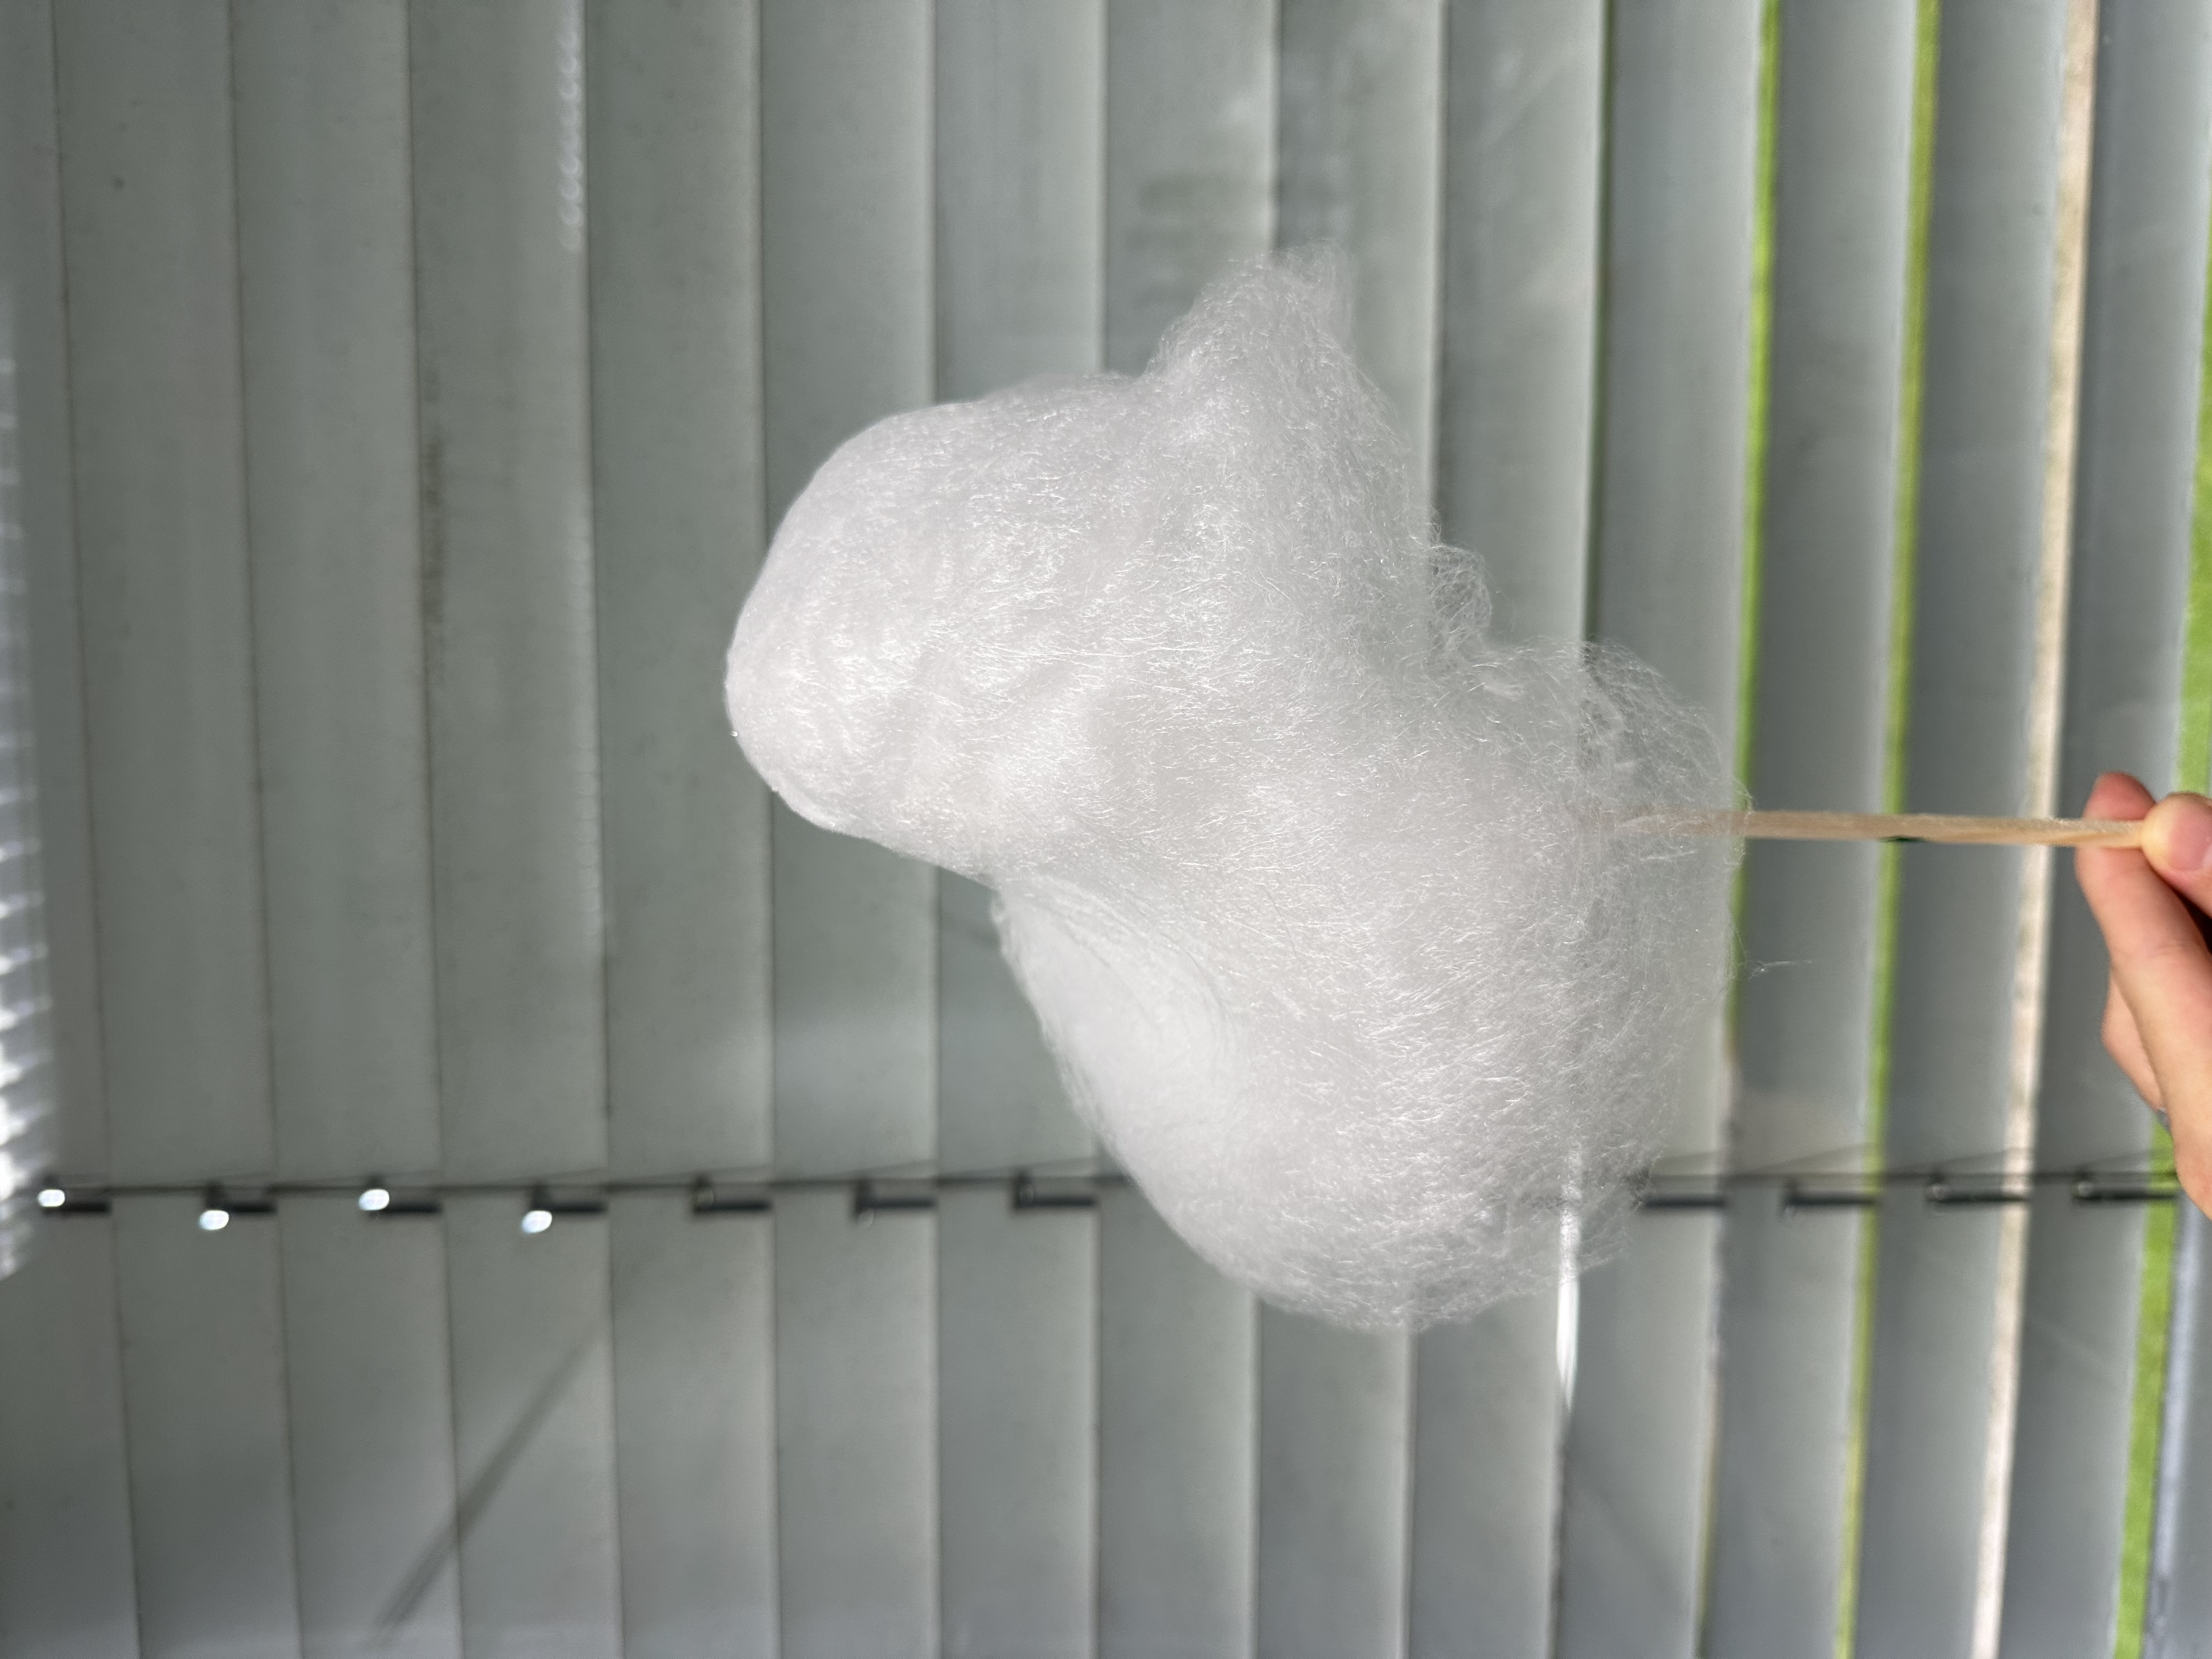
\includegraphics[width=\textwidth]{figures/firstCC.jpeg}
%         \caption{Actual cotton candy output}
%         \label{fig:cotton-candy}
% \end{figure}

\subsection{Volume Estimation}
% Stichpunkte:
% - You describe in detail how you estimate volume.
% - You assume the shape is an oblate spheroid (like a UFO).
% - You measure height and width with a ruler.
% - You apply the formula V = 4/3 * pi * a^2 * c
% - You derive a Fluffiness Index = Volume / Weight.

To approximate the spatial characteristics of the cotton candy output, the product was modeled as an oblate spheroid — a flattened ellipsoid shape that approximates the typical morphology observed during production.

\begin{figure}[H]
    \centering
    \begin{subfigure}[b]{0.45\textwidth}
        \centering
        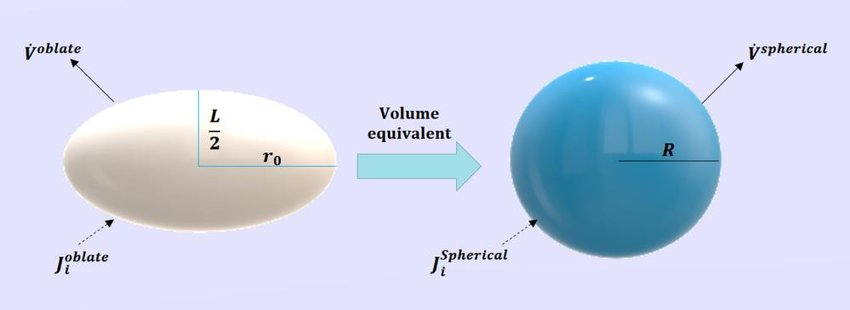
\includegraphics[width=\textwidth]{figures/Schematic-diagram-of-the-oblate-spheroid-and-its-volume-equivalent-sphere.jpg}
        \caption{Idealized oblate spheroid}
        \label{fig:oblate-spheroid}
    \end{subfigure}
    \hfill
    \begin{subfigure}[b]{0.45\textwidth}
        \centering
        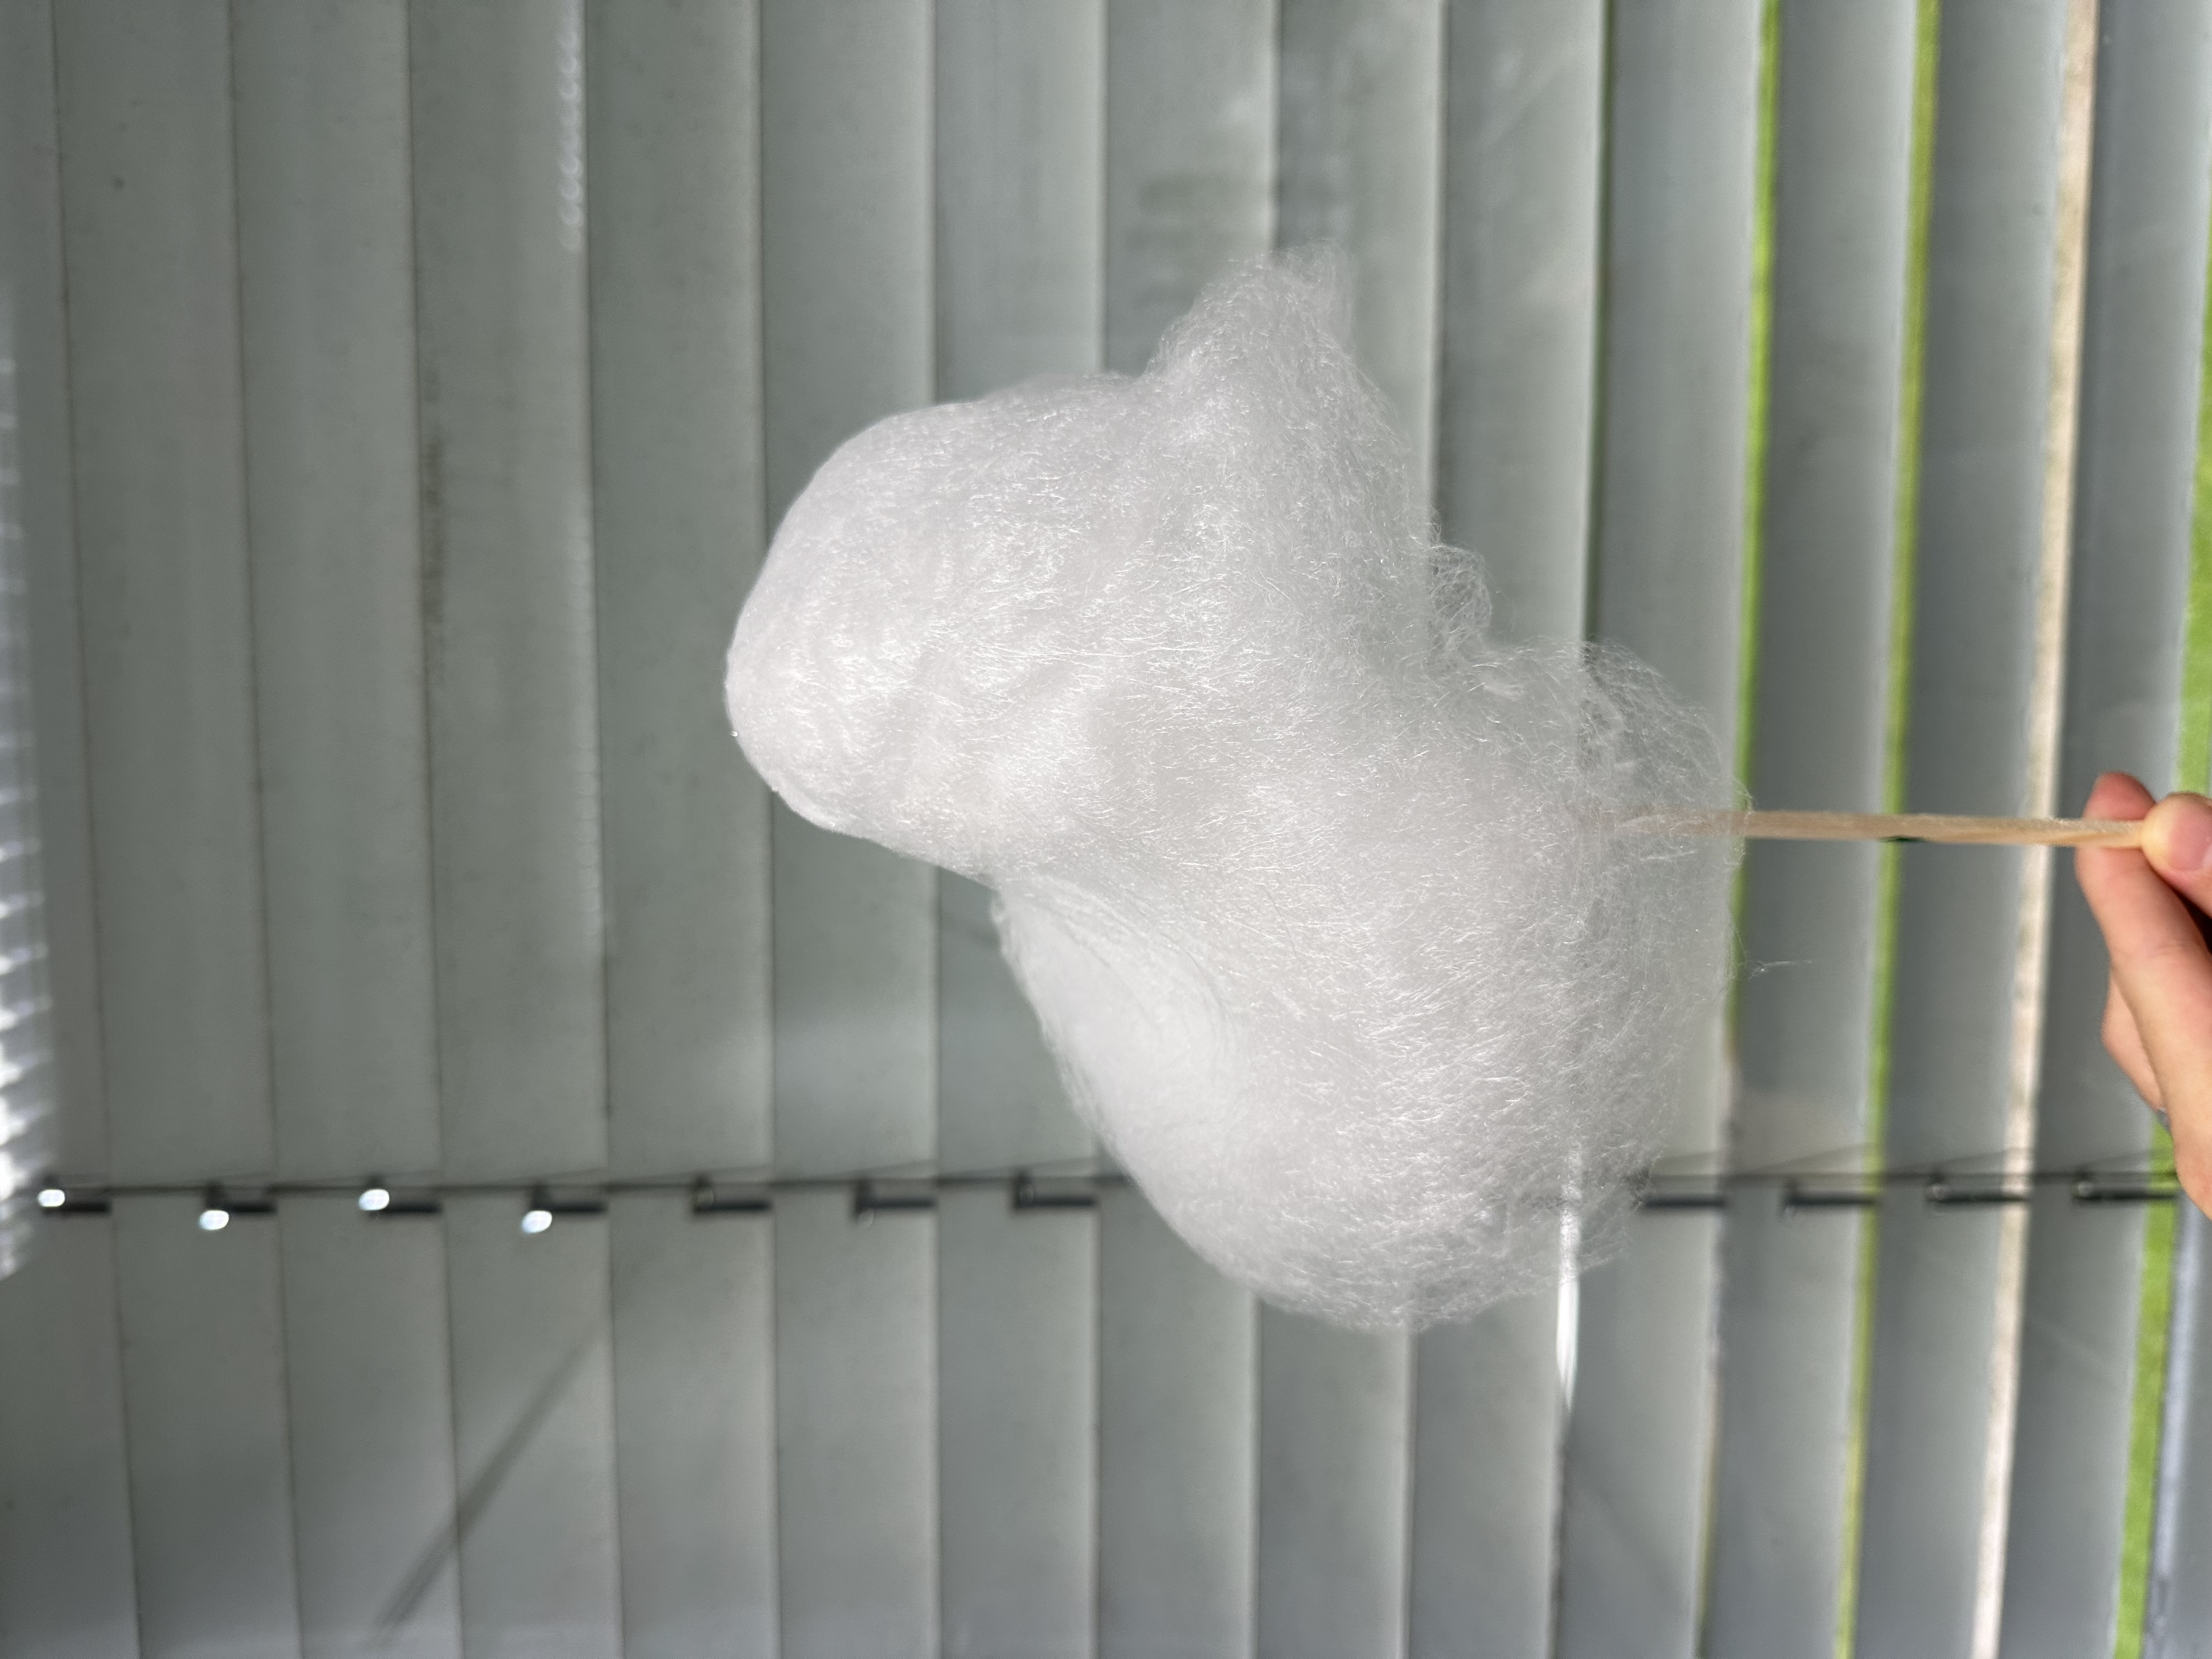
\includegraphics[width=\textwidth]{figures/firstCC.jpeg}
        \caption{Actual cotton candy output}
        \label{fig:cotton-candy}
    \end{subfigure}
    \caption{Comparison between geometric approximation and real cotton candy morphology}
    \label{fig:volume-comparison}
\end{figure}

Measurements of the maximum width and height were taken manually using a standard ruler immediately after each production run. Based on these dimensions, the volume \( V \) was estimated using the standard formula for an oblate spheroid:

\[
V = \frac{4}{3} \pi a^2 c
\]

where \( a \) is the equatorial radius (half of the width) and \( c \) is the polar radius (half of the height). Although this approach does not capture fine-grained structural variations, it offers a practical and repeatable method to compare volumetric differences across runs.

To further assess structural quality, a Fluffiness Index was derived as:

\[
\text{Fluffiness Index} = \frac{V}{\text{Weight}}
\]

This index serves as a proxy for the density of the cotton candy, with higher values indicating a lighter, airier structure. The same procedure and tools were applied consistently across all production runs to ensure internal comparability.

\subsection{Limitations in Volume Measurement}

The estimation of cotton candy volume relied on manual measurements of width and height, followed by geometric approximation. While this method provides a reasonable basis for comparative analysis, it is subject to several limitations: (a) the inherently irregular and fragile structure of cotton candy, (b) potential observer bias during manual measurement, and (c) the assumption of a regular geometric shape. As such, the absolute values of estimated volume should be interpreted with caution. However, because the same procedure was applied uniformly across all experimental runs, the relative differences and trends derived from this method remain valid for assessing the effects of the digital twin optimization.

\section{Pressure Functions}
Here I want to briefly show the pressure funcs we get from the scale and our implemented function, and why we decided not to use them (spoiler: To little time)


\section{Product Quality Measurement}
The development of an automated quality assessment system for cotton candy production presented significant challenges due to the inherently complex and variable nature of the product. Initial attempts to quantify cotton candy quality through traditional volumetric measurements proved unfeasible, as the product's form changes dramatically during the spinning process, making consistent volume measurements impractical within our laboratory constraints.

\subsection{Quality Assessment Approach}

Given the limitations of direct physical measurements, we established a ground-truth quality scoring system based on manual evaluation of the first 100 cotton candy samples. Each sample was assessed across three primary dimensions:

\begin{itemize}
    \item \textbf{Weight consistency}: Deviation from target weight parameters
    \item \textbf{Structural integrity}: Evaluation of cotton candy fluffiness and density
    \item \textbf{Overall form quality}: Categorical assessment (1-3 scale: poor, acceptable, good)
\end{itemize}

The manual scoring process was conducted systematically to minimize evaluator bias, with scores ranging from 0 to 75 points. This approach provided a consistent baseline for developing an automated quality prediction system.

\subsection{Algorithmic Quality Prediction}

To automate quality assessment, we used machine learning to predict quality scores from sensor measurements. The system uses three types of input data:

\begin{itemize}
    \item \texttt{touch\_pos1-3}: Contact positions when the robotic arm touches the cotton candy to measure its size at different heights
    \item \texttt{max\_pos1-3}: Pressure readings when moving the cotton candy down 5cm and back up, indicating structural strength
    \item \texttt{cc\_weight}: Final weight of cotton candy (without stick) from 12.65g sugar input
\end{itemize}

We developed a linear regression model with custom features based on our understanding of cotton candy quality. This process involved several key steps and discoveries:

\textbf{Understanding the Data:} Each cotton candy sample gives us seven measurements - three touch positions, three pressure readings, and one weight. The touch positions tell us how big the cotton candy is at different heights. When the robotic arm can touch the cotton candy close to the stick, it means the cotton candy is fluffy and well-formed. When it has to reach far out, the cotton candy is either too dense or poorly shaped.

\textbf{Smart Features:} We created mathematical formulas that capture what makes good cotton candy. Instead of just using raw measurements, we built features that understand cotton candy physics:
\begin{itemize}
    \item \textbf{Weight optimality:} We learned that 9--12 grams is the sweet spot for high-quality cotton candy. Too light means not enough sugar stuck to form proper structure, while too heavy indicates the presence of lumps from previous production runs, which creates an undesirable texture. Weights of 7--9 grams produce normal quality but receive lower scores, while anything below 7 grams indicates poor cotton candy formation.
    \item \textbf{Touch quality:} The touch position measurements work inversely---smaller distances (closer to the stick) indicate better structure and fluffiness. When the sensor reads 11, it means the robotic arm didn't make contact at all, representing the worst possible structure. The optimal range appears to be between 3--6, though the exact sweet spot within this range required empirical determination through our dataset. For the height (\texttt{touch\_pos2}), 6 means no contact at all.
    \item \textbf{Pressure patterns:} The way cotton candy resists being pushed down reveals its internal structure. Too little pressure (below 20 grams) indicates the cotton candy is overly fluffy with poor cohesion, while too much pressure (above 30 grams) suggests crystallization and density issues that reduce quality. The optimal pressure range of 20--30 grams indicates proper sugar fiber formation and structural integrity.
    \todo{cite the research that we did up that proves this}
\end{itemize}

\textbf{The First Problem - Training Bias:} Our initial approach had a major flaw. We only used data from successful production runs (iterations 56 and above) because we thought this would give us a "clean" dataset. This was a mistake. The algorithm learned to recognize good cotton candy but had never seen truly bad cotton candy during training. When we tested it on early production attempts, it consistently gave scores that were 30 points too high - it simply didn't know what failure looked like.

\textbf{The Solution - Complete Dataset Training:} We retrained the model using all 72 samples, including the early failed attempts where we were still learning how to operate the machine. This gave the algorithm experience with the full quality spectrum, from complete failures to perfect cotton candy. The improvement was dramatic - the bias problem disappeared.

\textbf{Why We Used All Data:} Unlike typical machine learning projects where you split data into training and testing sets, we used our complete dataset for training. This decision follows best practices for small dataset scenarios \cite{Zaki2020}. Since our goal was to build a production tool rather than prove the algorithm works on unseen machines, using all available data gave us the best possible model for our specific setup.

\textbf{Feature Selection Process:} We systematically tested which measurements actually helped predict quality. Some obvious candidates failed completely - for example, height measurements were inconsistent because cotton candy changes shape so easily. We kept only the features that showed reliable correlation with human quality judgments across all our samples.

\subsection{Validation Results}

The final algorithm achieved strong correlation with manual assessments (r = 0.853, MAE = 7.83 points). The correlation coefficient shows the algorithm captures about 73% of quality variation, while the mean absolute error represents roughly 10% deviation on our 0-75 point scale \cite{Zaki2020}.

Figure~\ref{fig:quality_comparison} shows the close match between predicted and actual quality scores across all production runs, validating our approach for automated quality control.

\begin{figure}[htbp]
    \centering
    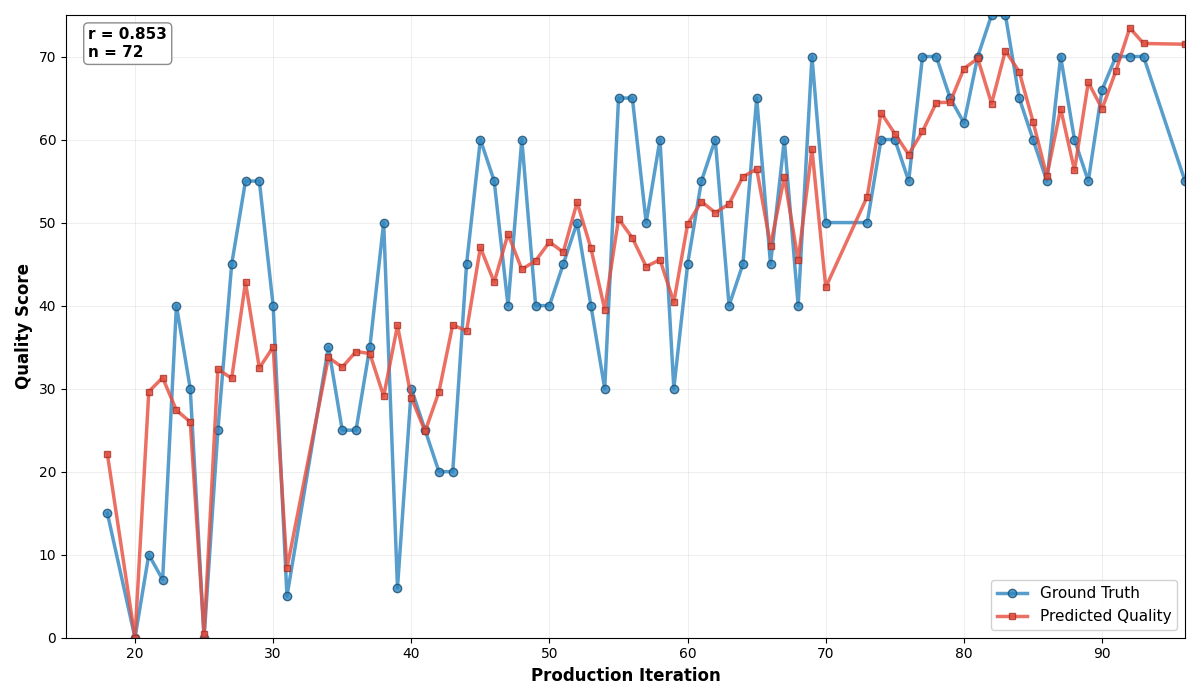
\includegraphics[width=1\textwidth]{figures/ground_truth_vs_score3_iterations.png}
    \caption{Comparison of manual quality scores (ground truth) and algorithmic predictions across production iterations. The strong correlation (r = 0.853) validates the automated quality assessment approach.}
    \label{fig:quality_comparison}
\end{figure}

The algorithm successfully captures both the learning progression evident in early iterations and the quality consistency achieved in later production runs, providing a reliable foundation for automated quality control in the digital twin system. This automated quality assessment eliminates the need for manual evaluation while maintaining assessment accuracy, enabling real-time quality monitoring and process optimization.


\section{Feature Engineering for Decision Tree Optimization}
\label{sec:feature-engineering}

To enable effective machine learning optimization, the raw process data was transformed into a structured feature vector suitable for decision tree modeling. This preprocessing involved careful selection and organization of variables to maximize predictive power while minimizing redundancy and computational complexity.

\subsection{Feature Vector Structure}

The final feature vector consists of 28 carefully selected features organized in a logical hierarchy:

\begin{enumerate}
    \item \textbf{Process Parameters (6 features):} Core decision variables including iteration since maintenance, wait time, cook time, cooldown time, and derived timing metrics (duration until handover and total duration)
    \item \textbf{Environmental Baseline (2 features):} External humidity and temperature captured at process initiation to establish ambient conditions
    \item \textbf{Internal Environmental Dynamics (20 features):} Four internal sensors measured across five critical process phases:
    \begin{itemize}
        \item Internal humidity (InH) and temperature (InT) sensors
        \item Infrared ambient temperature (IrA) at the sensor location
        %\item Infrared object temperature (IrO) of the rotating cotton candy machine head, which correlates with the actual internal head temperature (e.g., IrO = 81.55 corresponds to actual internal temperature ≈ 178°C, like we saw before)
    \end{itemize}
\end{enumerate}

\subsection{Redundancy Elimination Strategy}


Analysis of environmental sensor data revealed significant redundancy in external measurements, where external humidity and temperature remained virtually constant throughout the production process (±0.4\% and ±0.1°C variation respectively). To optimize the feature set:

\begin{itemize}
    \item \textbf{External sensors} were reduced from 10 measurements (2 sensors × 5 phases) to 2 baseline measurements, capturing ambient conditions without repetitive data
    \item \textbf{Internal sensors} were retained across all 5 phases, as they exhibited substantial variation (internal humidity: -27\% change, internal temperature: +15°C change, infrared ambient temperature and machine head object temperature: up to +58 units variation)
\end{itemize}

This optimization reduced the environmental feature space from 30 to 22 features while preserving all meaningful environmental dynamics, resulting in a 22\% reduction in feature dimensionality without information loss.

\subsection{Process Phase Identification}

Five critical process phases were identified for environmental monitoring:

\begin{enumerate}
    \item \textbf{Before turn-on:} Baseline internal conditions prior to machine activation
    \item \textbf{After flow start:} Environmental state during active cotton candy production
    \item \textbf{After flow end:} Conditions immediately following production completion
    \item \textbf{After weigh start:} Environmental state at cooling phase initiation
    \item \textbf{End:} Final environmental conditions post-cooling
\end{enumerate}

This temporal sampling strategy captures the complete thermal and humidity evolution during cotton candy production, enabling the decision tree to learn correlations between environmental conditions and process outcomes.

\section{Parameter Optimization Results}
\label{sec:parameter-optimization}

Through comprehensive analysis of the collected dataset using machine learning techniques (Random Forest, Extra Trees, and Gradient Boosting), we identified optimal parameter bounds for the three critical control variables. The analysis revealed that environmental humidity sensors (particularly before_turn_on_env_InH and during_flow_env_InH) are the most important quality predictors, followed by timing parameters.

\subsection{Optimized Parameter Bounds}

Based on the decision tree analysis of high-quality samples (quality score ≥ 70), the following parameter bounds were established:

\begin{itemize}
    \item \textbf{Wait Time:} 34--54 seconds (optimal: 44 seconds)
    \begin{itemize}
        \item Significantly reduced from initial default of 102 seconds
        \item Reduces energy consumption while maintaining quality
        \item Accounts for pre-heated machine state in continuous production
    \end{itemize}
    
    \item \textbf{Cook Time:} 66--77 seconds (optimal: 71 seconds)
    \begin{itemize}
        \item Reduced from initial default of 105 seconds
        \item Balances sugar caramelization with energy efficiency
        \item Prevents overcooking that leads to crystallization
    \end{itemize}
    
    \item \textbf{Cooldown Time:} 54--57 seconds (optimal: 55 seconds)
    \begin{itemize}
        \item Slightly reduced from default 60 seconds
        \item Prevents residual sugar burning in subsequent runs
        \item Optimizes cycle time for batch production
    \end{itemize}
\end{itemize}

\subsection{Environmental Adaptation Strategy}

For challenging environmental conditions (low humidity or temperature), the following parameter adjustments are recommended:

\begin{itemize}
    \item \textbf{Low Before Turn-On Conditions} (humidity ≤ 33\% or temperature ≤ 26°C):
    \begin{itemize}
        \item Wait Time: Increase to 45--50 seconds
        \item Cook Time: Increase to 72--75 seconds  
        \item Cooldown Time: Maintain 55--57 seconds
    \end{itemize}
\end{itemize}

These bounds represent a 32\% reduction in total cycle time compared to initial parameters while maintaining quality scores above 70 points.

\subsection{Production Phase Temperature Control}

Analysis of the machine head temperature during active cotton candy production revealed critical temperature thresholds for quality optimization. The infrared object sensor (\texttt{after\_flow\_start\_env\_IrO}) monitoring the spinning head temperature during sugar flow provides real-time feedback for production quality control.

\subsubsection{Optimal Temperature Bounds}

Machine learning analysis identified a narrow temperature window that produces consistently high-quality cotton candy:

\begin{itemize}
    \item \textbf{Target Range:} 74.5--76.0°C (optimal production temperature)
    \begin{itemize}
        \item Produces quality scores of 70+ points
        \item 42.1\% success rate for high-quality samples (≥65 points)
        \item Average quality score: 68.2 points in this range
    \end{itemize}
    
    \item \textbf{Acceptable Range:} 74.0--76.5°C (good quality zone)
    \begin{itemize}
        \item Maintains acceptable quality with minor variations
        \item Provides operational flexibility for temperature fluctuations
    \end{itemize}
    
    \item \textbf{Critical Thresholds:} < 70°C or > 77°C (intervention required)
    \begin{itemize}
        \item Below 70°C: Poor quality (average 33.1 points, 0\% high-quality rate)
        \item Above 76°C: Risk of overheating and sugar crystallization
    \end{itemize}
\end{itemize}

\subsubsection{Temperature Progression Analysis}

The analysis revealed optimal temperature progression patterns from machine startup to active production:

\begin{itemize}
    \item \textbf{Pre-production temperature:} 55--60°C (\texttt{before\_turn\_on\_env\_IrO})
    \item \textbf{Production temperature:} 74.5--76.0°C (\texttt{after\_flow\_start\_env\_IrO})
    \item \textbf{Temperature increase:} +15--19°C during transition to production
\end{itemize}

This temperature progression ensures proper sugar melting without overcooking, achieving optimal cotton candy formation.

\subsubsection{Real-time Temperature Control Strategy}

For implementation in the next 100 iterations, the following temperature control logic will be applied:

\begin{table}[htbp]
    \centering
    \caption{Production phase temperature control strategy}
    \label{tab:temp-control}
    \begin{tabular}{|l|l|l|l|}
        \hline
        \textbf{Temperature Range} & \textbf{Action} & \textbf{Quality Level} & \textbf{Strategy} \\
        \hline
        < 70°C & Increase heating & Poor & More heating \\
        70--74°C & Monitor closely & Moderate & Standard \\
        \textbf{74--76°C} & \textbf{Maintain} & \textbf{Excellent} & \textbf{OPTIMAL} \\
        > 76°C & Reduce heat & Risk zone & Cool down \\
        \hline
    \end{tabular}
\end{table}

This real-time temperature monitoring enables dynamic process adjustment to maintain optimal production conditions throughout each cotton candy cycle.

\subsection{Implementation for Next 100 Iterations}

The optimized parameter bounds will be implemented in the next 100 production iterations to validate their effectiveness in practice. The digital twin system will:

\begin{enumerate}
    \item Apply the parameter bounds as constraints in the decision tree optimization
    \item Monitor quality outcomes to confirm the 70+ quality score target is maintained
    \item Track energy consumption reduction compared to baseline parameters
    \item Collect additional environmental sensor data to refine the adaptation strategy
    \item Document any edge cases requiring parameter adjustments beyond the established bounds
\end{enumerate}

This implementation phase will serve as final validation that the machine learning-derived parameter optimization translates to consistent quality improvements in real-world production scenarios.

  \chapter{Evaluation}
\label{sec:evaluation}

\section{Product Output Quality}

Test for github of changing things here

% Stichpunkte:
% - You refer to the volume measurements to analyze quality.
% - You compare volume/fluffiness before and after optimization.
% - Do not repeat the formula or measurement steps here.

The quality of the cotton candy produced in each run was assessed using the previously introduced weight and volume-based metrics. In particular, changes in product volume and the derived Fluffiness Index were analyzed across multiple runs to evaluate whether the digital twin contributed to a measurable improvement in output quality.


/section{Product Output Consistency}
Like we saw in the research, the less the max pressure of the sugar the better quality the cotton candy.

the smaller the cc, the less quality (when count is )

After count >= 10 its a bad score (too small)
  \chapter{Discussion}
\label{sec:discussion}


  \chapter{Conclusion}
\label{sec:conclusion}

1-2 pages

% And finally Conclusion, where we summarize the key contributions of our work, and its significance in the broader context of digital twin research and applications.

% Restate the Motivation & Approach
% 	•	Start by briefly recalling why prescriptive digital twins matter (efficiency, sustainability, quality improvements).
% 	•	Emphasize that your work focused on building a bottom-up prescriptive digital twin for the Cotton Candy Automata.

% ⸻

% 2. Summarize Key Findings

% Answer each research question in a concise way:
% 	•	RQ1: The digital twin improved production quality, reduced energy use, and optimized time compared to the baseline “unintelligent” automata.
% 	•	RQ2: Analysis of process data revealed strong correlations (e.g., between heating time and candy texture, or sugar amount and production consistency), confirming that empirical parameter identification was effective.
% 	•	RQ3: By mapping the methodology to popcorn production, you showed that the bottom-up approach is transferable to other thermo-transformative processes, reinforcing its generalizability.
% 	•	RQ4: The prescriptive twin was able to recommend process adjustments, though environmental factors such as ambient humidity could not yet be controlled. These represent promising directions for future improvement.

% ⸻

% 3. Contributions
% 	•	Practical: A working prototype of a prescriptive digital twin for a robotic system, showing measurable efficiency and quality gains.
% 	•	Methodological: Demonstrated how a bottom-up, sensor-driven approach can be used to construct prescriptive digital twins, reducing the need for large historical datasets.
% 	•	Conceptual: Provided a transferable abstraction (inputs, controls, states, outputs, constraints) that aligns with the Research Manifesto on Digital Twins of Business Processes (Fornari et al., 2025) and can be applied in other domains.

% ⸻

% 4. Limitations
% 	•	Depended on one specific robotic system in a lab setting.
% 	•	Environmental factors (humidity, temperature) could only be observed, not manipulated.
% 	•	Scaling to more complex industrial processes would require integration with additional sensors and actuators.

% ⸻

% 5. Future Work
% 	•	Implementing environmental control (humidity/temperature) to test full prescriptive capabilities.
% 	•	Extending the methodology to other processes (e.g., roasting, baking, drying).
% 	•	Incorporating advanced AI techniques (e.g., reinforcement learning) for adaptive optimization, as recommended in the digital twin literature .
% 	•	Integrating human-in-the-loop features to improve explainability and usability.

% ⸻

% 6. Closing Statement

% Conclude with something like:

% Overall, this thesis demonstrates the feasibility and value of bottom-up prescriptive digital twins for small-scale production systems. By combining empirical process data with prescriptive decision-making, the approach contributes to more efficient, sustainable, and adaptive operations. Beyond the cotton candy use case, the findings highlight pathways for generalizing digital twin design to broader industrial contexts, offering a foundation for future research and real-world applications.

  \newpage
  \printbibliography[heading=bibintoc]
  \newpage
  \appendix
  \chapter{Appendix}

\begin{table}[h!]
  \begin{center}
    \caption{Your first table}
    \label{tab:table1}
    \begin{tabular}{l|c|r} % <-- Alignments: 1st column left, 2nd middle and 3rd right, with vertical lines in between
      \textbf{Value 1} & \textbf{Value 2} & \textbf{Value 3}\\
      $\alpha$ & $\beta$ & $\gamma$ \\
      \hline
      1 & 1110.1 & a\\
      2 & 10.1 & b\\
      3 & 23.113231 & c\\
    \end{tabular}
  \end{center}
  \floatfoot{A note describing the table.}
\end{table}

\newpage

\begin{figure}[h]
    \centering
    \caption{My Figure Caption}
    
\includegraphics[width=0.7\textwidth]{tum-resources/images/Universitaet_Flaggen.jpg}
    \floatfoot{A note describing the figure}
    \label{fig:ourFigure}
\end{figure}

\end{document}
